\beginsong{Der Lagerboogie}[by={}]
\beginverse
Wir \[E]laden Sie zum Boogie ein, dann bleiben Sie auch \[B7]fit. Wir singen eine Strophe vor und dann singt jeder \[E]mit.
\endverse

\beginchorus
Ja ja ja, tschu tschu, der Lagerboogie ist unser \[B7]Boogie-Woogie, tschu tschu tschu, die Zeit vergeht im \[E]Nu.
\endchorus

\beginverse
Und \[E]eins und zwei und drei und vier, und drei und zwei und \[B7]eins, der Text der ist ganz Schnuppe hier, die Hauptsache es \[E]reimt.
\endverse

\beginverse
Der \[E]Text kann noch viel dümmer sein, das macht uns gar nichts \[B7]aus, wir stimmen in das Liedchen ein und brüllen voll he\[E]raus.
\endverse

\beginverse
Der \[E]Adam sang den Boogie schon, den Boogie singen \[B7]wir. Der Boogie ist der beste Song, drum eins, zwei, drei und \[E]vier. 
\endverse

\beginverse
Im \[E]Pfarrhaus ist ein großer Krach, Herrn Pfarrer hört man \[B7]schon, denn jeden Morgen um halb acht, da singt er diesen \[E]Song.
\endverse

\beginverse
Die \[E]Kuh gibt Süß- und Sauermilch den lieben langen \[B7]Tag. Der Ochse dieses dumme Vieh gibt leider nur Spi\[E]nat.
\endverse

\beginverse
Es \[E]schreit die Geiß, es bellt der Hund, die Kuh brüllt dazu \[B7]muh, dem Vogel ist's schon lang zu bunt, er will jetzt seine \[E]Ruh'.
\endverse

\beginverse
Vom \[E]Boogie wackelt schon die Wand, die Scheiben fallen \[B7]aus und doch sind wir jetzt noch nicht still und singen voll he\[E]raus. 
\endverse

\beginverse
Wir \[E]haben nun genug geseh'n und wollen jetzt nach \[B7]Haus, wir wollen jetzt nach Hause geh'n so lasst und endlich \[E]raus. 
\endverse

\beginverse
Die \[E]kleine Möve Jonathan, die regt mich ganz schön \[B7]auf, drum nehm ich ihren Kopf und hau' ein paarmal feste \[E]drauf!
\endverse

\beginchorus
Ja ja ja, tschu tschu, der Lagerboogie ist unser \[B7]Boogie-Woogie, tschu tschu tschu, die Zeit vergeht im \[E]Nu.
\endchorus

\vspace{10mm}

\rule{\textwidth}{0.5pt}

\vspace{2.5mm}

\rule{\textwidth}{0.5pt}

\vspace{2.5mm}

\rule{\textwidth}{0.5pt}

\vspace{2.5mm}

\rule{\textwidth}{0.5pt}

\newpage

\mbox{}

\vfill

\centering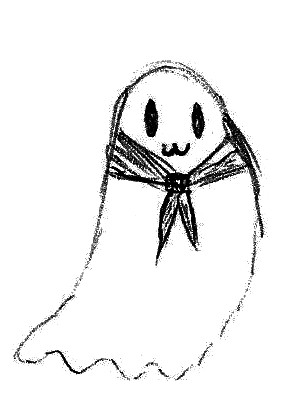
\includegraphics[width=4cm]{img/lagerboogie.jpg}

\vspace*{\fill}

\endsong
